%
%   K A D O N O
%   "kadono.tex"
%

\documentclass[10pt,b5paper,papersize,dvipdfmx]{jsbook}

\usepackage{vuccaken}
\usepackage{vuccaken2019}

% スタイルファイルの読み込みや自作マクロは、
% 最終的には vuccaken2019.sty の中に書いてください。
% とりあえずはここに書いてもらって構いません。


\begin{document} % 以下本文

% \mokuji{2} % 目次出力

% - - - - - - - - - - - - - - - - - - - - - - - - %
\kaishititle%
  {熱}% title
  {基礎理工学研究科 M 1回生}% 所属
  {\vname{門野}{広大}}% name
% - - - - - - - - - - - - - - - - - - - - - - - - %


\section*{はじめに}
熱って何?温度ってなに?どうやって熱は伝わっているの?そんな疑問に一生に一度は出会ったことがあると思います。実際熱の伝わり方というものをちゃんと理解しようとすると莫大な時間がかかりますし、不可逆なものでもあるのでそもそも理解できないのかもしれません。でも、限定的な条件において理解することは容易にできます。今回の会誌ではそんな物理の世界では常識的なことを主に書いていきたいと思います。\par
今回は状況が限定的な状態で、実際に人間が住んでいる環境とはかけ離れているため役に立たないと思われると思います。研究分野ではとても役にたちます。その理由を最後の方に私がやっている研究の話を含めて書きたいと思います。

% 熱って何?そもそも温度って何?熱伝導率って何で決まるの?物質のなに?格子ってなに?
% 格子振動って何?フォノンってなに?

%
\section{温度}




\section{フォノン君}
今回は気体、液体ではなく、固体の中の熱の流れについて考えようと思います。まず考えたいのが、固体の中でも、一つの原子のみで構成されている単結晶です。最初から三次元で考えるとよくわからなくなるので、原子同士がばねで一列につながっている状態を考えます(図\ref{fig:bane})。\par

\begin{figure}[htbp]
  \centering
  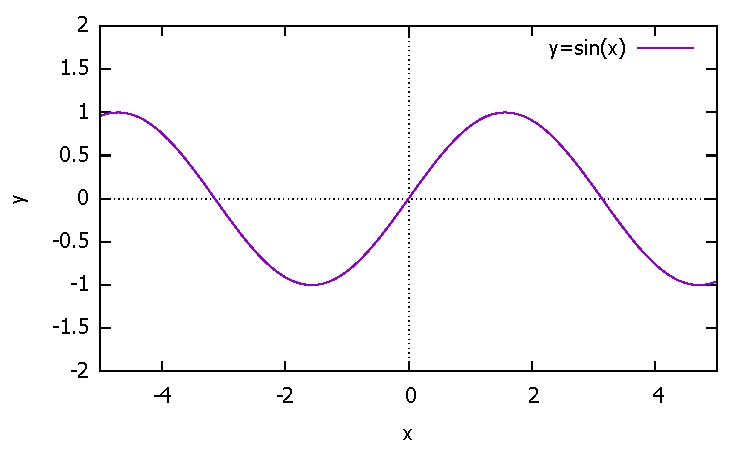
\includegraphics[width=10cm]{temp/fig-sin.pdf}
  \caption{一次元の結晶}
  \label{fig:bane}
\end{figure}
構成原子は最近接の間にだけ力を及ぼし会うと仮定します。$s$番目の原子の変位を$u_s$すると、$s$番目の原子の運動方程式は次のようにあらわされる。
\begin{align}
  M\frac{\mathrm{d}^2u_s}{\mathrm{d}t^2} = F_s = \alpha (u_{s+1} - u_s) - \alpha (u_s - u_{s-1})
  \label{eq:satom}
\end{align}
ここで、$M$は原子の質量、$\alpha$はばね定数、$F_s$は$s$番目の原子に及ぼす力。\par
式\ref{eq:satom}の解は波の式であると予測されます。波の式について少し話をしましょう。代表的な正弦波をあらわす式は
\begin{align}
  A(x) = A_0 \sin \left(\frac{2\pi x}{\lambda} + \phi \right)
\end{align}
とかけます。\par
ここで、波数$k$というものを導入すると、
\begin{align}
  A(x) = A_0 \sin (kx + \phi)
\end{align}
となります。波数$k (= 2\pi/\lambda)$は、単位長さあたりに含まれる1波長分の波の数に$2\pi$をかけた量である。さあ、ここで波数$k$というものをわざわざ導入しました。どうしてこんなものを導入するのか疑問に思う人がいると思います。大学では友達以上にであう波数$k$がどういうものを示しているのでしょうか。



\begin{align}
  u(\bm{r},t) = u_0 \exp(i(\bm{k} \cdot \bm{r} - \omega t))
\end{align}
ここで、$u_0$は振幅、$\bm{k}$は波数ベクトル、$\bm{r}$は位置ベクトル、$\omega$は角周波数。\par

\section{比熱とか熱伝導率とか}
ここからは、固体中の熱物性、特に比熱、熱伝導率、について書いていきたいと思います。
\subsection{比熱}
比熱について、まず比熱とは、1 kgの物質の温度を1 Kだけあげるのに必要な熱量として定義されいます。水の場合、比熱は$4.2 \times 10^3\  \mathrm{J\ K ^{-1} kg^{-1}}$なので、1 kgの水の温度を1 Kあげるためには$4.2 \times 10^3 J$だけの熱量が必要ということになります。これに対して、銅の比熱は$3.8 \times 10^2\ \mathrm{J\ K ^{-1} kg^{-1}}$と水の比熱の1/10以下である。つまり、銅の方が水よりも10倍温まりやすい。\par
固体の比熱について考えるためには統計力学の知識が必要ですが、それは参考文献に任せて次に進みます。比熱は、$\frac{\mathrm{d}U}{\mathrm{d}T}$
\subsection{熱伝導率}
\section{ちょっと変わった話}

\section{終わりに}
% \begin{figure}[htbp]
%   \centering
%   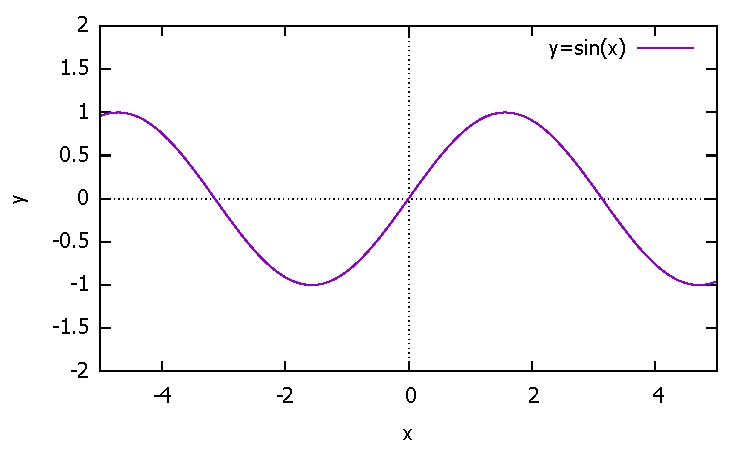
\includegraphics[width=10cm]{temp/fig-sin.pdf}
%   \caption{$y=\sin x$のグラフ。gnuplotで作成した。}
%   \label{fig:sin}
% \end{figure}

%% 参考文献
\begin{thebibliography}{99}
  \item 横田伊佐秋,『物理学テキストシリーズ 熱力学』,岩波書店,1987.
  \item 矢口裕之,『初歩から学ぶ固体物理学』,講談社,2017.
  \item W.COCHRAN・小林正一・福地充(訳),『固体物性シリーズ3 格子振動』,丸善出版,昭和50年.
  \item 田崎晴明,『新物理学シリーズ37 統計力学』,培風館,2008.
\end{thebibliography}

\end{document}
%
% ファイトだよ!
%